\documentclass[12pt,oneside]{book}
\usepackage{geometry}                		% See geometry.pdf to learn the layout options. There are lots.
\geometry{a4paper}                   			% ... or a4paper or a5paper or ... 
%\geometry{landscape}                		% Activate for for rotated page geometry
%\usepackage[parfill]{parskip}    		% Activate to begin paragraphs with an empty line rather than an indent
\usepackage{graphicx}				% Use pdf, png, jpg, or epsß with pdflatex; use eps in DVI mode
								% TeX will automatically convert eps --> pdf in pdflatex		
\usepackage{amssymb}

\usepackage[spanish]{babel}			% Permite que partes automáticas del documento aparezcan en castellano.
\usepackage[utf8]{inputenc}			% Permite escribir tildes y otros caracteres directamente en el .tex
\usepackage[T1]{fontenc}				% Asegura que el documento resultante use caracteres de una fuente apropiada.

\usepackage{hyperref}				% Permite poner urls y links dentro del documento

\title{Mi Juego Favorito}
\author{José Velez
\\Carlos Ramirez
\\Diego Cabrera}
%\date{}							% Activate to display a given date or no date

\begin{document}
\maketitle
\tableofcontents

\chapter{Introducción}
Este libro fue creado como una hherramienta colaborativa de archivo de texto plano. La herramienta que habilita dicha colaboración, en este taller, es Git.

\chapter{Los Juegos}

\section{Solitario}

\begin{figure}[htbp]
\begin{center}
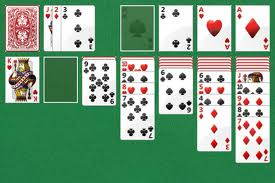
\includegraphics[width=.60\textwidth]{./imagenes/solitario.png}
\caption{Solitario}
\label{Solitario}
\end{center}
\end{figure}
Solitario\footnote{\url{http://solitariospider.org/}} es un juego de naipes o cartas, muy popular en todo el mundo. Precisamente, el nombre se refiere al hecho de que sólo hay un jugador en competencia. Es considerado como un juego de paciencia y destreza cuyo objetivo es utilizar todas las cartas de la baraja para construir las cuatro pilas de naipes clasificadas por pintas comenzando por los ases en orden ascendente.
\vfill

\subsubsection{¿Por qué es uno de mis juegos favoritos?}
\begin{itemize}
\item Solitario Spider. Consigue emparejar e ir eliminando todas las cartas, formando grupos en funcion de tipo de juego de solitario. Completa en juego limpiando el tablero de cartas y, en algunos casos, antes que se te agote el tiempo.
 
\begin{center}
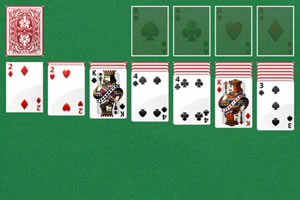
\includegraphics[width=.60\textwidth]{./imagenes/solitario2.png}
\label{Solitario2}
\end{center}
\end{itemize}

\section{Snake}

\begin{figure}[htbp]
\begin{center}
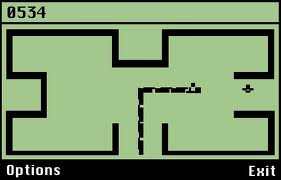
\includegraphics[width=.60\textwidth]{./imagenes/snake.png}
\caption{Snake}
\label{Snake}
\end{center}
\end{figure}
Snake\footnote{\url{http://www.snakegame.net/}} en este juego, el jugador controla una larga y delgada criatura, semejante a una serpiente, que vaga alrededor de un plano delimitado, recogiendo alimentos (o algún otro elemento), tratando de evitar golpear a su propia cola o las "paredes" que rodean el área de juego. Cada vez que la serpiente se come un pedazo de comida, la cola crece más, provocando que aumente la dificultad del juego. El usuario controla la dirección de la cabeza de la serpiente (arriba, abajo, izquierda o derecha) y el cuerpo de la serpiente la sigue. Además, el jugador no puede detener el movimiento de la serpiente, mientras que el juego está en marcha.

\vfill

\subsubsection{¿Por qué es uno de mis juegos favoritos?}
\begin{itemize}
\item Es uno de mis juegos favoritos porque mientras que la serpiente va comiendo, esta crece y la dificultad del juego aumentan, porque queda menos espacio para que la serpiente siga transitando.
Y además el juego cuenta con algunas variantes, que puede hacer que el juego aumente la dificultad y hacer más interesante el juego.

\begin{center}
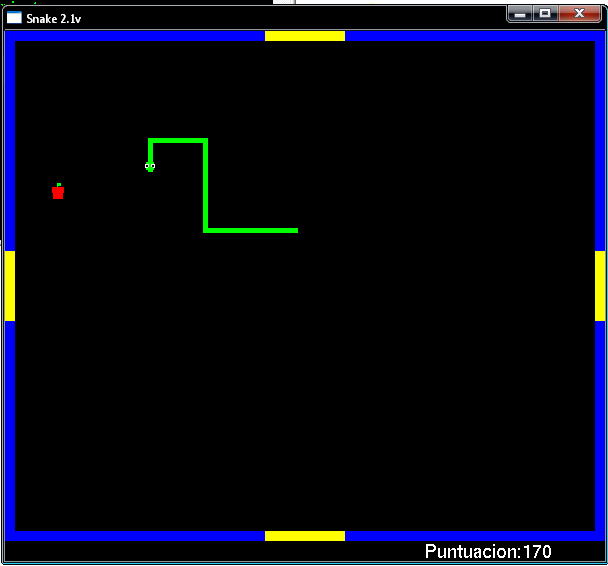
\includegraphics[width=.60\textwidth]{./imagenes/snake2.png}
\label{Snake2}
\end{center}

\end{itemize}

%\include{juegos/CallofDuty}

\chapter{Conclusiones}
Los juegos Solitario, Snake y Call of Duty son juegos muy populares; el Snake es un divertido juego adaptado en los teléfono Nokia que fueron unos de las primeras marcas en aparecer en nuestro país, el solitario es un juego de cartas donde debes ordenar las cartas desde el AS al REY, y se deben ordenar en forma descendente y alternando los colores, y Call of Duty es un juego de estrategia donde se simulas todas las guerras mundiales, donde debes estar alerta siempre.


\end{document}  
